%===============================================================================


%===============================================================================
%\documentclass[usenatbib, usegraphicx, letters]{mnras}
\documentclass[usenatbib, letters]{mnras}

%\usepackage{natbib}
\usepackage{graphicx}
\usepackage{hyperref}
%\usepackage{color}
%\usepackage{lscape}
%\usepackage{subfig}
%\citestyle{aa}
\usepackage{xspace}
% \usepackage{epsfig}
% \usepackage{amssymb}
% \usepackage{amsmath}
% \submitted{draft}
%\input{macros.tex}
\newcommand{\boldsymbol}[1]{\mbox{\boldmath{${#1}$}}}

\def\gammadm{\gamma_{\mathrm{DM}}}
\def\mdm{M_{\mathrm{DM}}}
\def\mhalo{M_{\mathrm{h}}}
\def\reff{R_{\mathrm{eff}}}
\def\rein{R_{\mathrm{Ein}}}
\def\ximin{\xi_{\mathrm{min}}}
\def\mtrue{M_*^{\mathrm{true}}}
\def\mchab{M_*^{\mathrm{Chab}}}
\def\msalp{M_*^{\mathrm{Salp}}}
\def\rhoc{\rho_c}
\def\aimf{\alpha_{\mathrm{IMF}}}
\def\loga0{\log{\alpha_0}}

\def\Sref#1{Section~\ref{#1}\xspace}
\def\Fref#1{Figure~\ref{#1}\xspace}
\def\Tref#1{Table~\ref{#1}\xspace}
\def\Eref#1{Equation~\ref{#1}\xspace}
%\addtolength\topmargin{1cm}

%===============================================================================

\begin{document}

\title{On how dry merges affect the effective stellar IMF of massive galaxies}
\author[Sonnenfeld et al.]{
Alessandro~Sonnenfeld,$^{1,2}$\thanks{E-mail:alessandro.sonnenfeld@ipmu.jp}
Carlo~Nipoti,$^{3}$
and Tommaso~Treu$^{2}$
\\
%$^{1}$Kavli Institute for the Physics and Mathematics of the Universe (WPI),The University of Tokyo Institutes for Advanced Study, The University of Tokyo, Kashiwa, Chiba 277-8583, Japan \\
$^{1}$Kavli IPMU (WPI), UTIAS, The University of Tokyo, Kashiwa, Chiba 277-8583, Japan \\
$^{2}$Department of Physics and Astronomy, University of California, Los Angeles, 430 Portola Plaza, Los Angeles, CA 90025, USA \\
$^{3}$Department of Physics and Astronomy, Bologna University, viale Berti-Pichat 6/2, 40127 Bologna, Italy
}

\maketitle

%-------------------------------------------------------------------------------
\begin{abstract}
The stellar IMF of early-type galaxies is the combination of the IMF of the stellar population formed in-situ and that of accreted stellar populations.
We introduce the concept of effective IMF, defined as the ratio between the true stellar mass of a galaxy and the stellar mass inferred assuming a Salpeter IMF, and present a theoretical model for its evolution as a result of dry mergers.
Using the dry merger evolution model from \citet{Nip++12} together with empirically motivated prescriptions for the IMF we make predictions for how the effective IMF of massive early-type galaxies changes between $z=2$ and $z=0$.
We find that trends of the IMF with stellar mass or velocity dispersion are preserved by dry mergers, but become less strong with time.
We also find that dry mergers can mix the dependence of the IMF on stellar mass and velocity dispersion
, making it challenging to infer what quantity regulates the IMF from $z=0$ observations of global galactic properties.
\end{abstract}

\begin{keywords}
   galaxies: elliptical and lenticular, cD -- galaxies: evolution
\end{keywords}

%-------------------------------------------------------------------------------
\section{Introduction}\label{sect:intro}

Undrstanding the origin of the stellar initial mass function (IMF) is currently one of the biggest challenges in galaxy formation theory.
Observational constraints on the IMF provide us with a puzzling scenario, where the IMF appears to be remarkably self-similar across different environments within the Milky Way \citep[see e.g.][]{BCM10}, while it is inferred to vary systematically as a function of mass in massive early-type galaxies \citep{Tre++10,Cap++12,CvD12,Spi++14}.
Efforts have been put into reproducing from a theoretical standpoint the observed IMF trends. However, despite recent progress \citep{H+C11,Kru11,Hop12,GKH15}, we still lack a coherent description of star formation across all environments.

One complication in comparing measurements of the IMF with models is that present day stellar populations are ensembles of stars formed a different epochs in a range of environments.
For massive early-type galaxies, a significant fraction of their present day stellar mass is believed to be accreted from other systems \citep{vDo++10}.
If the IMF is not universal, then each accreted object will in general have a different IMF from the preexisting population of the central galaxy.
The IMF of a massive galaxy at $z=0$ will then be combination of the IMF of the stellar population formed in-situ and that of the accreted galaxies.
How does this "effective" IMF evolve in time?

In this work we model the evolution of the effective IMF of massive galaxies from $z=2$ to the present.
We adopt a simple prescription for assigning the starting IMF of an ensemble of galaxies and then evolve the stellar population of central galaxies by merging their stellar content with that of accreted satellites.
We tune our model to match the observed IMF-stellar mass trend at $z=0$ and use it to make predictions on the stellar IMF at higher redshifts.

The paper is organized as follows.  In \Sref{sect:model} we describe our model for the IMF of $z=2$ galaxies and its evolution as a result of dry mergers.
In \Sref{sect:results} we show our predictions on the time evolution of the IMF.
We discuss and summarize our results in \Sref{sect:discuss}.

%%%%%%%%%%%%%%%%%%%%%%%%%%%%%%%%%%%%%%%%%%%%%%%%%%%%%%%%%%%%%%%%%%%%%%%%%%

\section{The model}\label{sect:model}

\subsection{Parameters and notation}
Throughout our work we use the following quantities to describe the stellar content of our galaxies. We first define a true stellar mass, $\mtrue$. Then we introduce a Salpeter stellar mass, $\msalp$, defined as the stellar mass one would infer by fitting a stellar population synthesis model based on a Salpeter IMF to broad-band photometric data. This quantity is typically used when observationally measuring stellar masses.
We then introduce an {\em IMF mismatch parameter}
\begin{equation}\label{eq:aimf}
\aimf = \frac{\mtrue}{\msalp}.
\end{equation}
Stellar populations with a more bottom-light IMF than a Salpeter IMF will have $\alpha<1$. A Chabrier IMF for example corresponds typically to a value $\aimf\approx0.6$.
As defined above, $\aimf$ is a well-defined quantity also for galaxies that do not have a homogeneous stellar population, for example as a result of mergers.

In addition to the stellar mass of a galaxy, we track its halo mass $\mhalo$ and its central velocity dispersion $\sigma$.
Stellar mass, halo mass and stellar velocity dispersion are the only quantities that enter our model.

\subsection{The mock sample}

We generate a sample of halo masses at $z=2$ drawn from the halo mass function described by \citet{Tin++08}, using an upper cut off at $\log{M_h} < 13.5M_\odot$.
We make this cut to focus on the regime of galaxy or galaxy group scale halos, where most observational constraints on the IMF are measured, excluding cluster of galaxy environments.
We then assign a Salpeter stellar mass to each halo using a stellar to halo mass relation (SHMR) from \citet{Lea++12}, including scatter.
We make an additional cut in stellar mass keeping only galaxies with $\log{\mchab} > 10.5$ and then select a random sample of 100 objects.
Finally we assign central velocity dispersions using the $M_*-\sigma$ relation measured by \citet{Aug++10} for low-z objects, generalized to higher redshifts ($z \sim 2$) following \citet{Mas++15}:
\begin{equation}\label{eq:mason}
\log{\sigma} = \sigma_0 + \beta_\sigma(\log{\mchab} - 11) + \zeta_\sigma\log{(1 + z)}.
\end{equation}



\subsection{The IMF}
\label{ssect:imfform}

The IMF of massive galaxies has been shown to correlate with stellar velocity dispersion \citep[e.g.]{Tre++10, CvD12, LaB++13, Spi++14, Pos++15}, stellar mass \citep{Aug++10b, Son++15}, mass-to-light ratio \citep{Cap++12} and stellar mass density \citep{Spi++15}.
In light of these observations, we adopt a relation of the following form for assigning the IMF to our model galaxies at $z=2$:
\begin{equation}\label{eq:imfform}
\log{\aimf} = a_*(\log{\mchab} - 11) + a_\sigma(\log{\sigma} - 2.3) + b.
\end{equation}
We then choose two different sets of values for the parameters $a_*$, $a_\sigma$ and $b$. In the first prescription, labeled ``$M_*$ model'', we set $a_*=0.26$, $a_\sigma=0$ and $b=0.11$.
For the second prescriprion, labeled ``$\sigma$ model'', we set $a_*=0$, $a_\sigma=1.00$ and $b=-0.06$.
In other terms, the first model is a power-law relation between IMF and stellar mass, with no residual dependence on $\sigma$, while vice-versa the IMF of the second model is set uniquely by the velocity dispersion.
In each model, the values of the parameters have been tuned to reproduce the low-z IMF measurements from \citet{Son++15}. Details on these measurements are given in \Sref{sect:obs}.

These prescriptions are purely empirically motivated. While there have been attempts at predicting the stellar IMF from first principles in terms of the global properties of a galaxy \citep[e.g.]{Kru11,Hop12}, implementing such models would require us to make additional assumptions on parameters of the star forming gas such as the pressure and the turbulence Mach number.
Given the current uncertainty on the true mechanism determining the IMF, the benefits of employing such theoretically motivated recipes are modest and we therefore limit our model to simpler empirical recipes.
%We show that the main results of this study hold for a range of different prescriptions for assigning the IMF.


\subsection{The dry merger evolution}

Our central galaxies are evolved to $z=0$ using the dry merger evolution model developed by \citet{Nip++12}, with a few modifications.
The method can be summarized as follows.
For each central galaxy we compute the evolution in its halo mass  using the following expression from \citet{FMB10}, which is derived from the Millennium I and II simulations:
\begin{equation}
\frac{\mathrm{d}\ln{\mhalo}}{\mathrm{d}z} = - \frac{\dot{M}_0}{10^{12}M_\odot H_0}\frac{1 + fz}{1 + z}\left(\frac{\mhalo}{10^{12}M_\odot}\right)^{g-1},
\end{equation}
with $\dot{M}_0 = 46.1 M_\odot \rm{\, yr}^{-1}$, $f=1.11$ and $g=1.1$.
In this step we are assuming that the growth history of each halo in our sample is the same as the average growth history for halos of the same mass.
We separate the growth in halo mass into smooth accretion and growth due to mergers. We estimate the latter with the following expression from \citet{FMB10},
\begin{equation}\label{eq:nmerg}
\frac{\mathrm{d}^2N_{\mathrm{merg}}}{\mathrm{d}z \mathrm{d}\xi}(z, \xi, \mhalo) = A\left(\frac{\mhalo}{10^{12}M_\odot}\right)^\alpha \xi ^\beta \exp{\left[\left(\frac{\xi}{\tilde{\xi}}\right)^\gamma\right]}(1 + z)^{\eta'},
\end{equation}
which describes the number of mergers between halos of mass ratio $\xi$ per unit redshift interval.
Following \citet{FMB10}, we assume $A=0.0104$, $\tilde{\xi}=9.72\times10^{-3}$, $\alpha=0.133$, $\beta=-1.995$, $\gamma=0.263$ and $\eta'=0.0993$.
At each timestep $dz$, the change in halo mass due to mergers is then the following integral over mergers of different halo mass ratios $\xi$,
\begin{equation}
\left[\frac{\mathrm{d}\ln{\mhalo}}{\mathrm{d}z}\right]_{\mathrm{merg}} = -\int_{\ximin}^1 \mhalo(x)\xi \frac{\mathrm{d}^2N_{\mathrm{merg}}}{\mathrm{d}z \mathrm{d}\xi} d\xi.
\end{equation}
We are assuming that only mergers with mass ratio larger than a minimum value $\ximin$ contribute. This minimum value is set by the merging time-scale: mergers with very small values of $\xi$ have merging time-scales larger than the age of the Universe and therefore cannot contribute to the accreted mass. We set $\ximin=0.03$ following \citet{Nip++12} and refer to that work for a more detailed discussion on the choice of this parameter.

We then calculate the growth in Salpeter stellar mass assuming that each accreted halo is associated with a stellar mass given by the (redshift dependent) SHMR of \citet{Lea++12}, and that this stellar mass is also accreted by the central galaxy:
\begin{equation}
\frac{\mathrm{d}\msalp}{\mathrm{d}z} = \int_{\ximin}^1 \mathcal{R}_{*,h}(\xi \mhalo, z)\xi\mhalo\frac{\mathrm{d}^2N_{\mathrm{merg}}}{\mathrm{d}z \mathrm{d}\xi} d\xi,
\end{equation}
where $\mathcal{R}_{*,h}$ is the SHMR. With this equation we are assuming that each merger event brings in exactly the average amount of stellar mass for its halo mass: in other words we are neglecting scatter in the merger history.

Each merger, in addition to increasing the mass of the galaxy, contributes to modify its velocity dispersion. Using the virial theorem under the assumption of parabolic orbits, \citet{NJO09} showed that the ratio between the {\em virial} velocity dispersion after and before a merger event of mass ratio $\xi$ is given by
\begin{equation}
\frac{\sigma_{v,f}^2}{\sigma_{v,i}^2} = \frac{1 + \xi\epsilon}{1 + \xi},
\end{equation}
where $\epsilon = \sigma_{v,a}^2/\sigma_{v,i}^2$ is the ratio between the velocity dispersion of the accreted object and that of the central galaxy, squared.
We then make the assumption that the stellar velocity dispersion of central and satellite are proportional to their virial velocity $\sigma \propto \sigma_v$, through which we can write the change in stellar velocity dispersion due to mergers as
\begin{equation}
\frac{\mathrm{d}^2\sigma^2}{\mathrm{d}z\mathrm{d}\xi} = \sigma^2\left[\frac{1 + \xi\epsilon}{1 + \xi} - 1\right]\frac{\mathrm{d}^2N_{\mathrm{merg}}}{\mathrm{d}z \mathrm{d}\xi}.
\end{equation}
We describe the velocity dispersion of the satellites with a relation between stellar mass and $\sigma$ of the form given by \Eref{eq:mason}, with no scatter. The values of the coefficients $\sigma_0$, $\beta_\sigma$ and $\zeta_\sigma$ are determined by fitting \Eref{eq:mason} to the $\msalp-\sigma$ relation of the central galaxies, and are updated at each timestep as the centrals evolve.

Finally, we need to describe the growth in true stellar mass for our centrals, which in turn requires to define the IMF of the accreted satellites.
Similarly to the velocity dispersion case, we assign the IMF of satellites using \Eref{eq:imfform}, where the coefficients are determined at each timestep by fitting the distribution of IMF as a function of stellar mass and velocity dispersion of the centrals.

We do not keep track of the spatial distribution of stars within our galaxies. Although observations could in principle detect spatial variations in IMF within a galaxy and put interesting constraints on IMF differences between the in-situ population and that of the accreted stars, that is beyond the scope of this work.


\section{Reference IMF measurements}\label{sect:obs}

The main goal of this work is to make predictions on the distribution of the IMF in massive galaxies as a function of redshift, using low-redshift observations as a reference point.
We choose the IMF measurements from \citep{Son++15} to be such reference point.
In this Section we summarize the main results of that work and carry out some additional analysis needed in order to calibrate our models to the observations.

\citet{Son++15} measured the stellar IMF for a sample of 80 early-type galaxies using strong lensing in combination with velocity dispersion data to constrain the stellar mass $\mtrue$ of each object.
Measurements of $\aimf$ for individual objects are very noisy. To cope with the low signal-to-noise of individual measurements, \citet{Son++15} combined them with a hierarchical Bayesian inference approach, in which they modeled the distribution of IMF normalization of the population of massive galaxies as a Gaussian and allowed the mean of such Gaussian to be a function of redshift, stellar mass and projected stellar mass density.
The analysis yielded the detection of a positive trend between the effective IMF and stellar mass and no detection of a dependence on redshift or stellar mass density.

The \citet{Son++15} analysis did not explore dependences between velocity dispersion and IMF, which we consider in our model.
Moreover, the relations between stellar mass and IMF explored by \citet{Son++15} were based on $\mtrue$, instead of $\msalp$.
For this reason we re-analyse here the \citet{Son++15} sample and fit for a dependence of the IMF on $\msalp$ and $\sigma$, as well as redshift. We then describe the distribution in effective IMF of the \citet{Son++15} sample of galaxies as a Gaussian with mean
\begin{equation}\label{eq:sl2sfit}
\mu_{\mathrm{IMF}} = a_z(z - 0.3) + a_*(\log{\msalp} - 11.5) + a_\sigma(\log{\sigma} - 2.4) + b
\end{equation}
and dispersion $s$. We fit for the parameters $a_z$, $a_*$, $a_\sigma$ and $s$ using a similar hierarchical Bayesian inference method as the one used by \citet{Son++15}.
Details of the fitting procedure are given in the Appendix.
In \Fref{fig:sl2scorner} we plot the posterior probability distribution for the parameters describing the IMF, marginalized over the other model parameters (which include parameters describing the dark matter distribution).
%
\begin{figure*}
 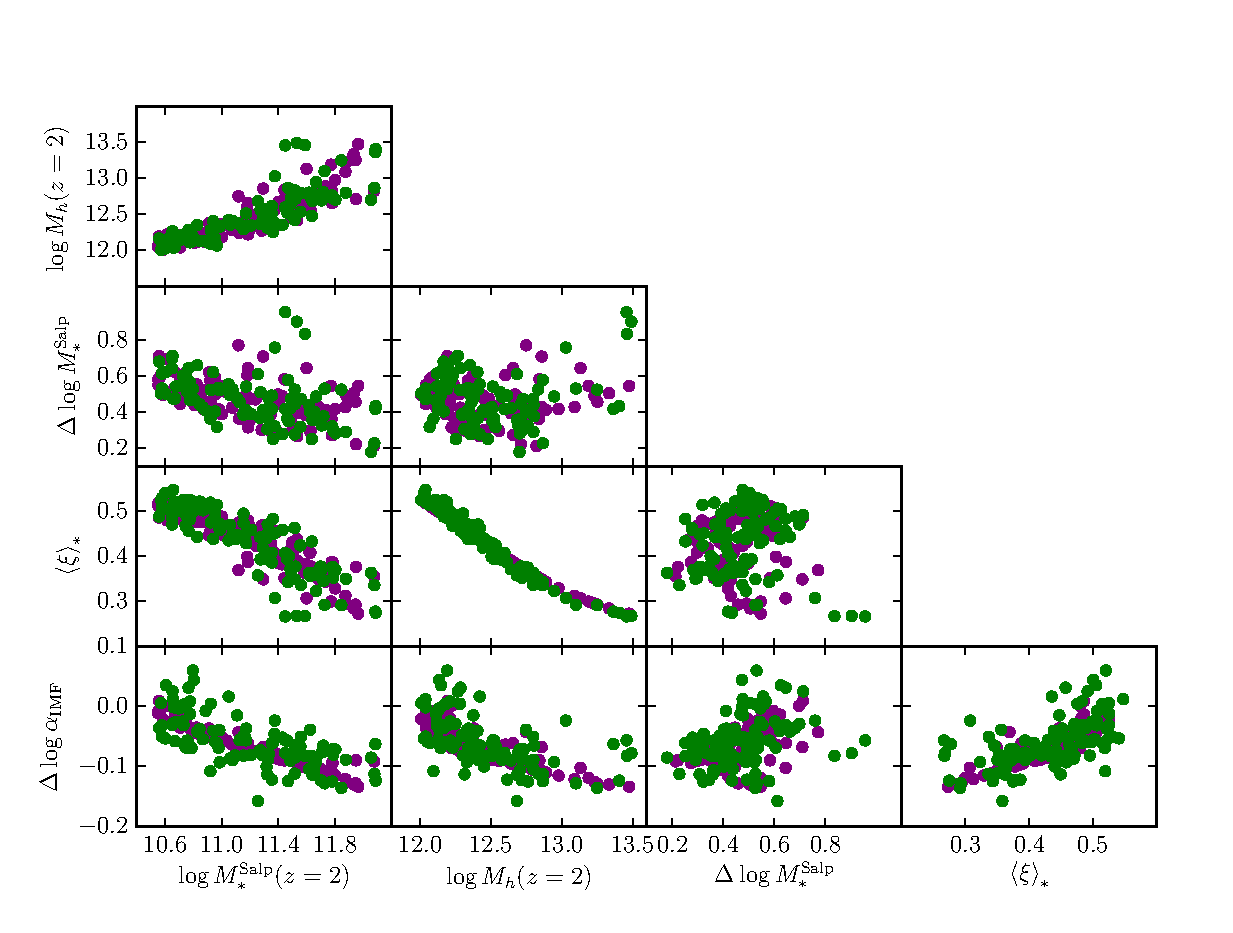
\includegraphics[width=\textwidth]{cornerplot.eps}
 \caption{{\em Purple dots}: ``$M_*$ model''. {\em Green dots}: ``$\sigma$ model''
}
 \label{fig:cornerplot}
\end{figure*}



%Since the sample of galaxies covers the redshift range $0.1 < z < 0.8$, we also allow for a redshift dependence of the IMF.

\subsection{Hierarchical Bayesian inference}
We use a similar hierarchical Bayesian inference method as the one used by \citet{Son++15} to fit for the distribution in IMF of the same sample of galaxies. The method can be summarized as follows.
We assume that the density profile of early-type galaxies can be described by the sum of a stellar component with a de Vaucouleurs profile and a dark matter component with a Navarro Frenk and White \citep{NFW97} profile.
We parametrize this model in terms of the Salpeter stellar mass $\msalp$, effective radius $\reff$, projected dark matter mass within a cylinder of radius $5$ kpc $\mdm5$, dark matter scale radius $r_s$, effective IMF $\aimf$.
Following \citet{Son++15} we fix $r_s = 10\reff$ for simplicity.
We then describe the {\em distribution} of galaxy parameters as the product of three terms:
\begin{equation}
\mathrm{I}(\msalp, \reff, \sigma, z)\mathrm(\mdm5, \aimf | \msalp, \reff, \sigma, z)
\end{equation}




through which they constrained the average IMF normalization of the population of massive galaxies and its dependence on redshift, stellar mass and stellar mass density.
The main finding of that analysis was that the IMF correlates strongly with stellar mass while the measurements are consistent with no dependence on stellar mass density and redshift, at fixed stellar mass.

\citet{Son++15} modeled the dependence between
Here we repeat the hierarchical inference analysis 

modeled the distribution of IMF in massive galaxies as a Gaussian in $\log{\aimf}$ with a mean 

%%%%%%%%%%%%%%%%%%%%%%%%%%%%%%%%%%%%%%%%%%%%%%%%%%%%%%%%%%%%%%%%%%%%%%%%%%

\section{Results}\label{sect:results}

In \Fref{fig:snap} we plot the IMF mismatch parameter for our mock sample of galaxies at three different redshifts ($z=2$, $z=1$ and $z=0$), as a function of stellar mass and velocity dispersion, for each model.
At each redshift snapshot we fit \Eref{eq:mstarmodel} and \Eref{eq:sigmamodel} to the mock data with a least-squares method. Best-fit curves are overplotted in \Fref{fig:snap}.
%
\begin{figure*}
 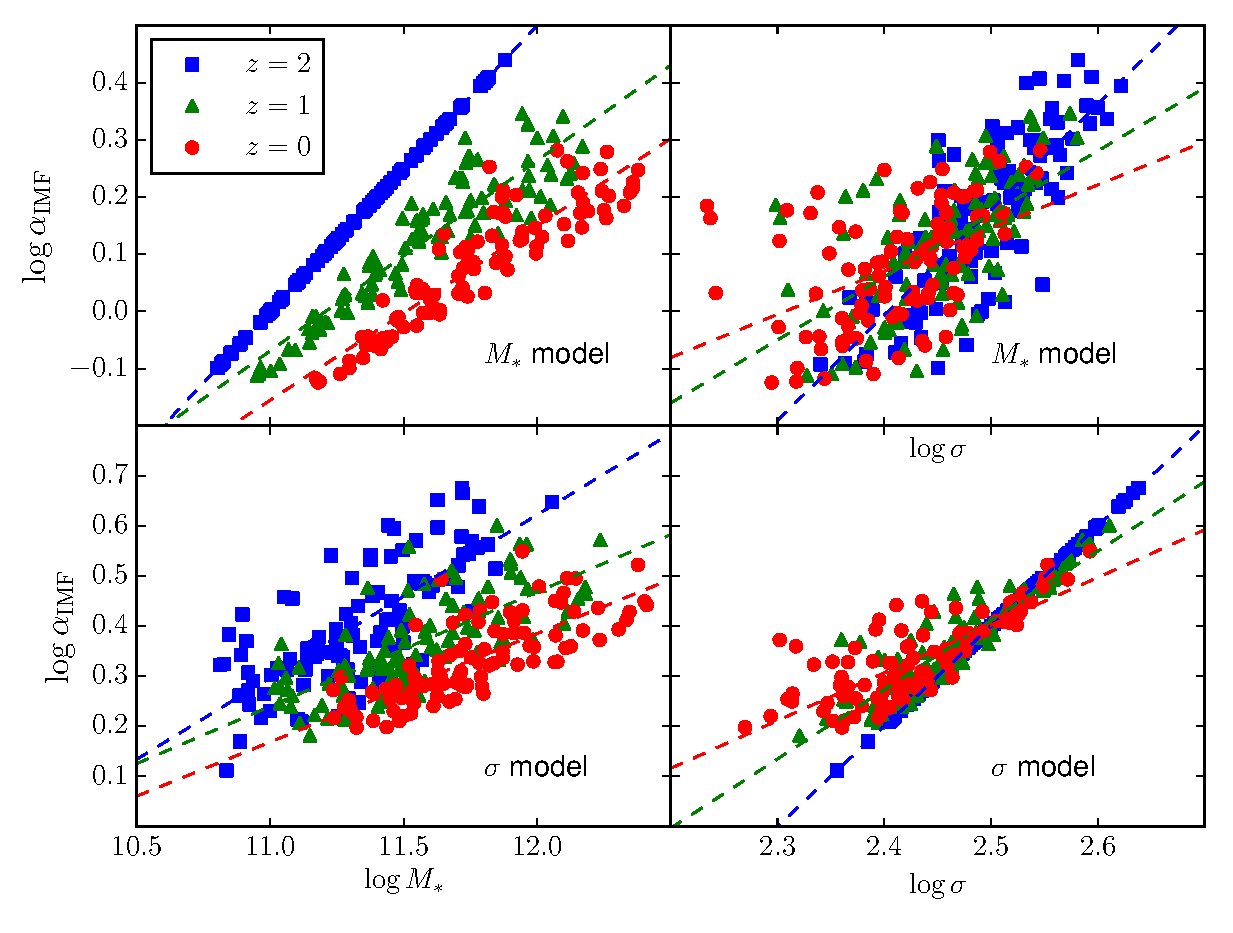
\includegraphics[width=\textwidth]{snapshots.eps}
 \caption{ IMF mismatch parameter $\aimf$ as a function of stellar mass ({\em left panels}) and central velocity dispersion ({\em right panels}) for the ``$M_*$ model'' ({\em top panels}) and ``$\sigma$ model'' ({\em bottom panels}) IMF recipes, at three different redshifts.
{\em Dashed lines:} Linear fit to the data in each redshift snapshot.
{\em Shaded regions:} Observational constraints from \citet{Son++15} ({\em left panels}) and \citet{Pos++15} ({\em right panels})
}
 \label{fig:snap}
\end{figure*}
%
\begin{table}
 \caption{Best-fit parameters of \Eref{eq:mstarmodel} and \Eref{eq:sigmamodel} to the mock data shown in \Fref{fig:snap}. The third number in each set represents the residual scatter around the best fit relation.}
 \label{tab:oneparfit}
 \begin{tabular}{lcc}
 \hline
 Data set & Eq. \ref{eq:mstarmodel} fit & Eq. \ref{eq:sigmamodel} fit\\
 & $(a_*, b_*, s_*)$ & $(a_\sigma, b_\sigma, s_\sigma)$ \\
 \hline
% ``$M_*$ model'', $z=2$ & $(0.35, 0.07, 0.)$ & (2., -0.1, 0.1) \\
 ''$M_*$ model'' & (0.26, 0.21, 0.00) & (1.06, 0.06, 0.06)\\
''$M_*$ model'' & (0.21, 0.13, 0.02) & (1.06, 0.06, 0.04)\\
''$M_*$ model'' & (0.20, 0.06, 0.02) & (1.08, 0.05, 0.04)\\
''$\sigma$ model'' & (0.24, 0.19, 0.05) & (1.20, 0.03, 0.00)\\
''$\sigma$ model'' & (0.19, 0.11, 0.04) & (1.06, 0.05, 0.01)\\
''$\sigma$ model'' & (0.18, 0.05, 0.03) & (1.02, 0.05, 0.01)\\

 \hline
 \end{tabular}
\end{table}

As can be seen by comparing the left hand panels in \Fref{fig:snap} with the right hand panels, correlations between IMF and stellar mass correspond to similar correlations with velocity dispersion, and vice-versa. This is just a consequence of the tight correlation between galaxy stellar mass and velocity dispersion in the mock sample (and in observations). 
Trends of $\aimf$ with stellar mass and velocity dispersion, which we assumed in place at $z=2$, are mostly preserved by dry mergers down to $z=0$, but become less steep with time.

By $z=1$ a relatively large scatter is introduced in the $\aimf-\sigma$ space (right hand panels of \Fref{fig:snap}), even for the ``$\sigma$ model'' where the sample is initialized at $z=2$ with zero scatter. This is mostly driven by the evolution of galaxies in the most massive halos: these objects experience the highest merger rates and their change in velocity dispersion is correspondingly high. %We will discuss this point more in the next Section.

For a given row in \Fref{fig:snap}, a look at the $z=2$ scatter plots in stellar mass and velocity dispersion space allows us to immediately identify which IMF recipe was used to produce the mock data.
The same procedure becomes non-trivial at $z=0$ due to scatter.
In order to test how accurately observations can discriminate between the two scenarios, we now perform fits in which the IMF can depend both on stellar mass and velocity dispersion:
\begin{equation}\label{eq:hybrid}
%\log{\aimf} = \frac{\partial \log{\aimf}}{\partial \log{M_*}}(\log{M_*} - 11) + \frac{\partial\log{\aimf}}{\partial\log{\sigma}}(\log{\sigma} - 2.3) + \log{\alpha_0}.
\log{\aimf} = a_*(\log{M_*} - 11) + a_\sigma(\log{\sigma} - 2.3) + b.
\end{equation}
In \Fref{fig:tracks} we plot the measured values of $a_*$ and $a_\sigma$ at each timestep.
In addition to the ``$M_*$ model'' and ``$\sigma$ model'' described above we also test a ``Hybrid model'' in which the IMF depends both on stellar mass and velocity dispersion as described by \Eref{eq:hybrid}, 
with $a_*=0.2$, $a_\sigma=1.5$, $b=0.0$.
%
\begin{figure}
 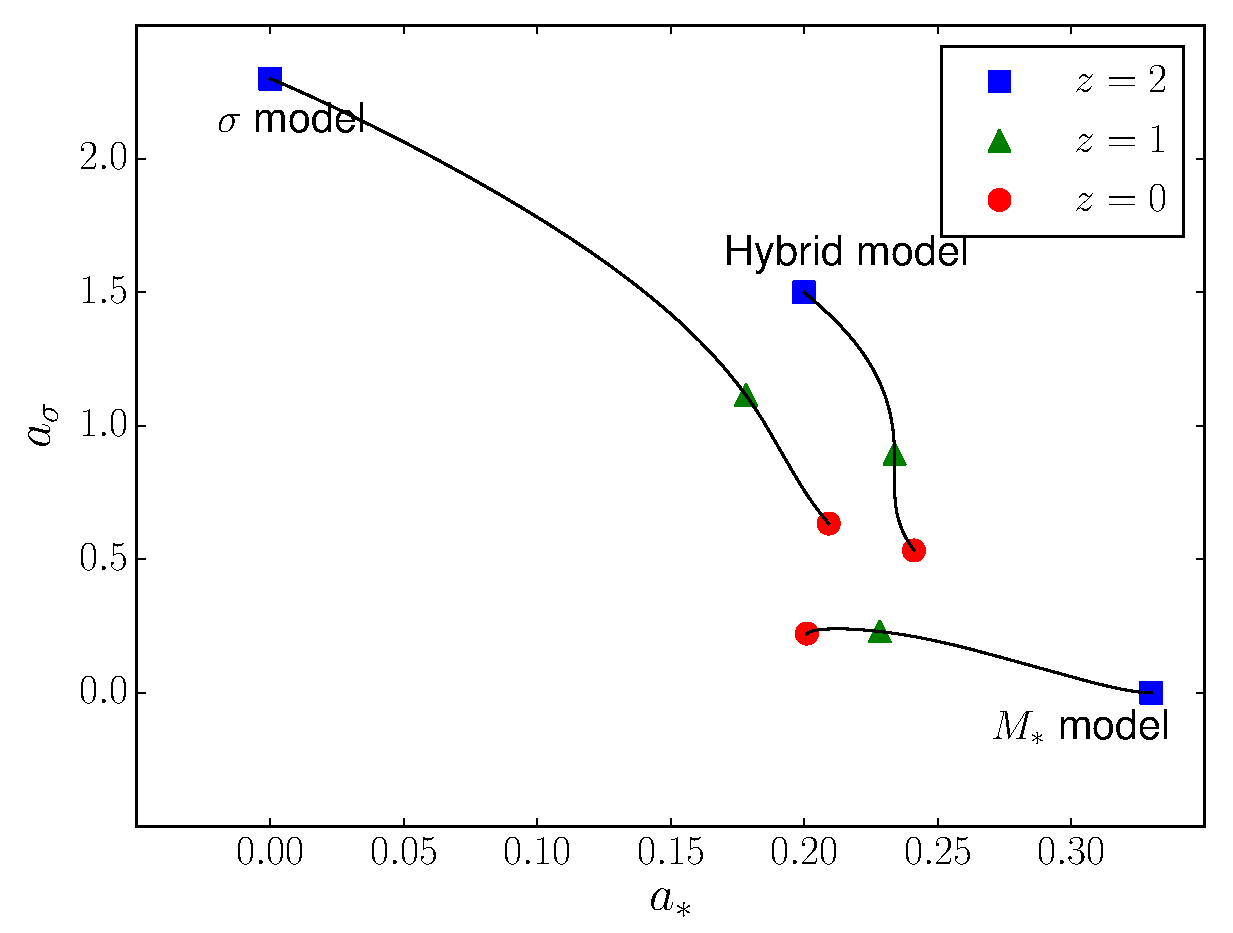
\includegraphics[width=\columnwidth]{tracks.eps}
 \caption{ 
Coefficients $a_*$ and $a_\sigma$, describing the dependence of the effective IMF on stellar mass and velocity dispersion, obtained by fitting \Eref{eq:hybrid} to mock data generated with the ``$M_*$ model'', ``$\sigma$ model'' and ``Hybrid model'' prescriptions at each timestep.
}
 \label{fig:tracks}
\end{figure}
%
The starting ($z=2$) point in the $a_*-a_\sigma$ space is by construction very different for the three mock sets. However by $z=0$ the tracks corresponding to the different models converge to intemediate values of $a_*$ and $a_\sigma$, meaning that, for the three models tested here, the $z=0$ effective IMF appears to depend both on stellar mass and velocity dispersion regardless of the starting point.


%One of the goals of observational studies of the IMF in massive galaxies is to determine which, among the global properties of galaxies, is the fundamental quantity the IMF appears to depend on.

%Assuming that the IMF is fundamentally determined by one (or a small set of) global property of agalaxy, we would ideally like to observationally identify that 
%Ideally we would like to observationally determine which, among the global properties of galaxies, is the fundamental quantity the IMF depends on, if present at all
%Ideally, we would like to observationally determine what global quantity the IMF fundamentally depends on, if present at all



\section{Discussion and Summary}\label{sect:discuss} 

Using empirically motivated recipes for describing the IMF of massive galaxies together with the dry merger evolution model developed by \citet{Nip++12} we studied the time evolution of the effective IMF, defined as the ratio between the true stellar mass and the stellar mass one would infer assuming a Chabrier IMF, of a population of massive galaxies from $z=2$ to $z=0$.
The models were set up to match the observed correlations between IMF and stellar mass and velocity dispersion in massive early-type galaxies at $z\sim0$.
Qualitatively, the trends imposed at $z=2$ are preserved with dry mergers. Quantitatively, we find that the amplitude of the correlations between effective IMF and galaxy stellar mass or velocity dispersion decreases with time.

To understand the origin of this evolution, in \Fref{fig:cornerplot} we plot the fractional change in effective IMF between $z=2$ and $z=0$, $\Delta\log{\aimf}=\log{\aimf}(z=0)-\log{\aimf}(z=2)$ of our mock galaxies together with key quantities such as the initial halo mass and initial stellar mass and accreted stellar mass. 
%
\begin{figure*}
 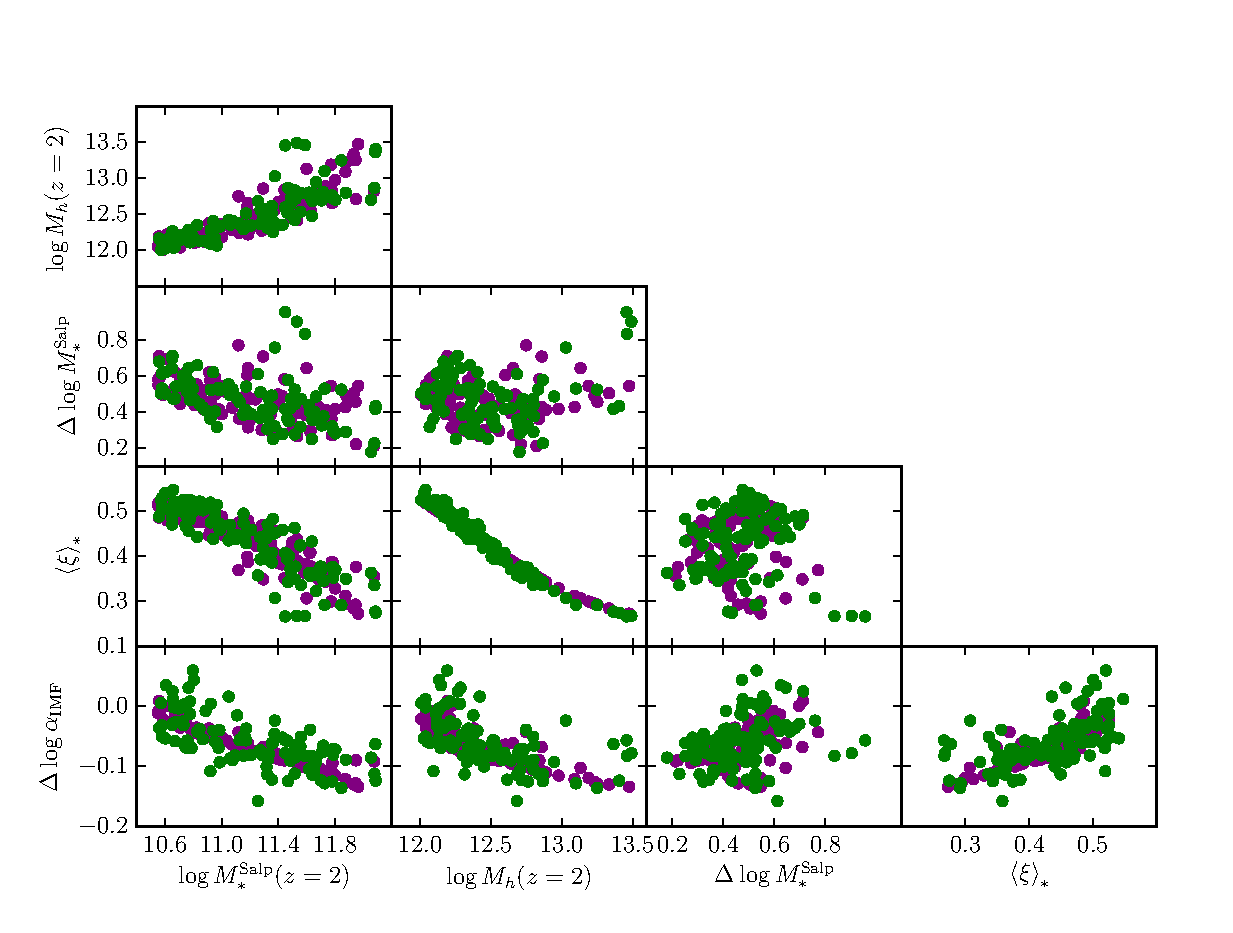
\includegraphics[width=\textwidth]{cornerplot.eps}
 \caption{{\em Purple dots}: ``$M_*$ model''. {\em Green dots}: ``$\sigma$ model''
}
 \label{fig:cornerplot}
\end{figure*}
%
The effective IMF of individual galaxies in our sample generally decreases with time ($\Delta\log{\aimf}<0$). This is easily understood, as by definition central galaxies merge with less massive systems that, in our model, have a less heavy IMF. 
In order to produce a dependence of the IMF on mass that becomes shallower with time, it is necessary for the more massive systems to have a stronger decrease in their IMF with time (more negative values of $\Delta\log{\aimf}$).
As can be seen in the bottom left panel of \Fref{fig:cornerplot}, this is indeed the case.

Differences in $\Delta\log{\aimf}$ reflect differences in merger history.
Since mergers tend to decrease the effective IMF normalization, we expect galaxies with the highest increase in stellar mass to also show the largest changes in effective IMF. However this is not observed to be the case, as can be seen from \Fref{fig:cornerplot} (fourth row, third column).
If the amount of accretion does not play a central role in setting the final IMF, then the different change in IMF between low mass and high mass systems must be set by differences in the type of mergers. To quantify this, we measure the accreted stellar mass-weighted merger mass ratio, $\left< \xi \right>_*$, defined as the average over all mergers between $z=2$ and $z=0$ of the halo mass ratio between the accreted satellites and the central halo weighted by the accreted stellar mass with each merger. $\left< \xi \right>_*$ is also plotted in \Fref{ref:cornerplot}. We see that $\left< \xi \right>_*$ increases for decreasing halo and stellar mass.
This means that for the most massive galaxies the bulk of the accreted stellar mass is brought in through mergers of relatively small mass ratio, while for less massive galaxies major mergers play a more important role.
Given our IMF prescription, where the heaviness of the IMF of satellites increases with mass, minor mergers produce a stronger decrease in the effective IMF of a galaxy than major mergers at fixed accreted stellar mass. 
This is seen in the bottom right panel of \Fref{fig:cornerplot}, where $\left< \xi \right>_*$ correlates with the change in effective IMF.
We then conclude that the shallowing of the $M_*-\aimf$ or $\sigma-\aimf$ trends with time seen in our \Fref{fig:snap} is a result of the different relative importance of major and minor mergers in systems at the 

A few systems at the low mass end of the distribution show an increase in the effective IMF normalization ($\Delta \log{\aimf} > 0$), apparently at odds with expectations. Although at $z=2$ any merger will produce a decrease in IMF normalization, as time goes by and galaxies grow it becomes possible for them to accrete satellites with stellar mass larger than their original mass at $z=2$. Since in our model the IMF of satellites does not evolve with time, these major mergers will then bring in galaxies with a heavier IMF than the central, hence the positive $\Delta\log{\aimf}$.

Another prediction of our model is the mixing between stellar mass and velocity dispersion dependence of the IMF shown in \Fref{fig:tracks}.
The (small) dependence of velocity dispersion, $a_\sigma$, seen at $z=0$ in the ``$M_*$ model'' can be easily understood. At $z=0$, at fixed stellar mass, we find galaxies with a range of initial stellar masses at $z=2$. Those with a larger $z=2$ stellar mass have a slower growth by definition, a heavier $z=2$ IMF by construction and a larger $z=2$ velocity dispersion on average. The ranking in $\sigma$ and $\aimf$ between those systems is roughly preserved by the dry merger evolution. Therefore at fixed $z=0$ stellar mass, objects with larger velocity dispersion will also have on average a heavier IMF.

The emergence of the stellar mass dependence in the ``$\sigma$ model'' is instead due to the distortion of the $\sigma-\aimf$ relation at $z=0$, apparent in the bottom right panel of \Fref{fig:snap} where the trend in IMF flattens at the low-$\sigma$ end. A model in which the IMF depends both on $\sigma$ and $M_*$ is simply a better fit to the data. 

An important assumption in our model is that all of the growth in stellar mass between $z=2$ and $z=0$ is due to dry mergers. In other terms, our model only applies to the population of quiescent galaxies at $z=2$. This assumption complicates the comparison between predictions from our model and observations, because the number density of quiescent galaxies is observed to increase substantially with time, in particular at $z>1$ \citep[e.g.][]{Ilb++13, Cas++13}. Depending on what the IMF of the newly quenched object is, some results might change as a result of the so-called progenitor bias. However: predictions on the $z<1$ evolution for the high-mass end of the galaxy distribution should still hold, since the number density of quiescent galaxies shows little evolution in that region of the parameter space \citep{Lop++12}.

%Another assumption we made is not allowing scatter in the merger history, as this is set by the halo mass. We tested this assumption by adding a 20% scatter in the merger rate and a scatter of $0.02$ in the allowed minimum merger mass ratio. No significant differences were found with respect ot the case with no scatter. 

To summarize, we predicted the evolution of the IMF in massive galaxies between $z=2$ and $z=0$ assuming a purely dry merger evolution.
We find that trends between stellar mass and velocity dispersion are qualitatively preserved by dry mergers, but the amplitude of the correlations decreases with time. 
At fixed stellar mass, we find that the IMF normalization decreases by $0.06\div0.08$ dex between $z=1$ and $z=0$ (depending on the prescription used). Current constraints from strong lensing on the redshift dependence of the IMF are consistent within $2-\sigma$ \citep[parameter $\zeta_{\mathrm{IMF}}$ of]{Son++15}.
Finally, we find that the relative dependence of the IMF on stellar mass and velocity dispersion gets mixed by dry mergers, making it difficult to observationally determine the fundamental parameter(s) governing the IMF from $z=0$ measurements.



%\section{Conclusions}\label{sect:concl} 

\section*{acknowledgments}
%-------------------------------------------------------------------------------

%\acknowledgments

% Boilerplate:
%\input{acknowledgments2.tex}

%-------------------------------------------------------------------------------

\bibliographystyle{mnras}
\bibliography{references}
%-------------------------------------------------------------------------------


\end{document}

%===============================================================================
